\documentclass[UTF8,a4paper,10pt]{ctexart}

% \documentclass[UTF8,a4paper,10pt]{article}
% \usepackage{xeCJK}
% \setCJKmainfont{SimSun}
% \setmainfont{Times New Roman}%英文字体

\usepackage[left=2.50cm, right=2.50cm, top=2.50cm, bottom=2.50cm]{geometry}
\usepackage{times}
\usepackage{amsmath, amsfonts, amssymb} % math equations, symbols
\usepackage[english]{babel}
\usepackage{color}      % color content
\usepackage{graphicx}   % import figures
\usepackage{url}        % hyperlinks
\usepackage{bm}         % bold type for equations
\usepackage{algorithm}
\usepackage{algorithmic}
\usepackage{indentfirst}
\usepackage{subfigure}
\setlength{\parindent}{2em}

\usepackage{tikz,mathpazo}
\usetikzlibrary{shapes.geometric, arrows}
\usetikzlibrary{calc}

\title{\textcolor[rgb]{0,0.3,0.6}{\textbf{基于经验和机器学习方法的遗传算法作曲探索 }\\ [2ex] \begin{large} Exploring\  of\  Genetic\  Algorithm\  Composition\  Based\  on\  Experience\ and\ Machine\  Learning\ Methods\end{large}}}
\author{关震岳\  李宇轩\  林潇涵\  胡泽昕\  张天越\  施朱鸣}
\date{\today}

% \documentclass[12pt,AutoFakeBold]{article}%第二个参数解决宋体没有粗体的问题
\usepackage{booktabs}%绘制三线表
% \usepackage{fontspec}%控制字体
% \usepackage[version=3]{mhchem}%化学反应式
% \usepackage{xeCJK}%控制中文字体
% \usepackage{latexsym}%绘制特殊数学符号
% \usepackage[a4paper]{geometry}%纸张大小和页边距
% \usepackage{pdfpages}%插入pdf页面
% \usepackage{titlesec}%控制标题格
% \usepackage{graphicx, epstopdf}%此处使.eps文件可转化成.pdf并应用自动编号功能
% \usepackage[journal=angew]{chemstyle}%此处设置图式的样式
% \usepackage{siunitx}%数学模式中使用SI单位
% \usepackage{color}%提供颜色支持
% \usepackage{listings,xcolor}
% \usepackage{amsfonts}
% \usepackage{indentfirst}

% \geometry{left=2.5cm,right=2.5cm,top=2.5cm,bottom=2.5cm}%页边距设置
% \setmainfont{Times New Roman}%英文字体
% \setCJKmainfont{SimSun}%中文字体
% \newfontfamily\arial{Arial}%Arial字体
% \XeTeXlinebreaklocale "zh"%中文自动换行
% \XeTeXlinebreakskip = 0pt plus 1pt%中文自动换行

\begin{document}
    \maketitle

    % % cover
    % \vspace*{4cm}
    % \begin{center}
    %     \Huge{\textbf{高压油管压力控制的数学模型}}
    % \end{center}
    % \vspace*{5cm}
    % \rule{\textwidth}{1mm}
    % \large{    
    % \textbf{摘要}\quad 对高压油管中的燃油注入和喷出的数学模型的建立,是研究和改善燃油发动机工作状况的必要前提。在本问题中,我们考察了一个由高压油泵、高压油管、喷油嘴和减压阀等部件组成的简单高压油路系统。我们将复杂的高压油路系统建立成一个形式简单而统一的数学形式
    % \[\frac{\dif p}{E\dif t}=\frac{Q_{in}-Q_{out}}{V}\]
    % 并从这个简洁优美的式子,推导出关于这个高压油路的控制理论依据。\\
    % \textbf{关键词}\quad 高压油管\quad 压力控制\quad 数学模型\\
    % }
    % \rule{\textwidth}{1mm}
    % \newpage

    \noindent \rule{\textwidth}{.625mm}
    \textbf{摘要}\quad 适应度函数的选取是遗传算法作曲的核心。本文中,我们报道了基于乐理经验知识构建适应度函数的方法,并且提出了一种基于机器学习方法构造适应度函数的方法。我们通过机器学习来提取旋律中的特征,以训练出的分类器将旋律划分为“好”的概率作为适应度函数,以此去除经验适应度函数的主观性。我们给出了基于逻辑斯蒂回归、多层感知机、随机森林和卷积神经网络模型构造的适应度函数,用遗传算法生成了例曲,并分析了机器学习模型选择对生成乐曲的影响。\\
    \textbf{关键词}\quad 机器学习\quad 遗传算法\quad 作曲\\
    \rule{\textwidth}{.625mm}
    \vspace*{.5cm}

    利用计算机进行算法作曲的尝试可以追溯到1956年Lejaren Hiller报道的弦乐四重奏作品llliac,而如今,遗传算法已经成为一种主要的算法作曲方法。遗传算法是一种模仿自然选择、适者生存的算法,算法的输入为一系列亲代样本,对它们进行随机变异操作,生成一系列子代,再使用适应度函数评估亲代和子代的集合中各个个体对环境的适应度,选取其中适应度最高的若干个个体,组成下一个亲代,如此循环,直到适应度收敛为止。适应度函数的选取是决定生成乐曲风格和质量的主要因素。\par
    本文中,我们将讨论遗传算法作曲的基本框架,并就适应度函数的具体实现进行深入讨论。我们将探讨两大类适应度函数的构造,其中一种基于乐理知识经验,另一种基于机器学习方法。

    \section{\textcolor[rgb]{0,0.3,0.6}{遗传算法作曲程序的基本框架}}%没写完

    我们对具体音乐建立了计算机模型,将音乐的最小单元确定为1个16分音符,8分音符视作两个相连的16分音符,以此类推。于是我们就实现了对音乐的编码,用一个整数数组储存一段音乐的音高,忽略强度。我们采取对音乐中随机某一个位置变成另一个音高的方法实现变异算法。对于生成的子代,为了提高迭代效率,我们放弃了轮盘赌算法,使用了贪心法,将子代和亲代放在一起,直接对他们按照适应度数值进行排序,取前若干个样本作为下一代的亲代。下面我们将就适应度函数的具体实现进行探讨。


    % 流程图定义基本形状
    \tikzstyle{startstop} = [rectangle, rounded corners, minimum width = 2cm, minimum height=1cm,text centered, draw = black, fill = black!10]
    \tikzstyle{io} = [trapezium, trapezium left angle=70, trapezium right angle=110, minimum width=2cm, minimum height=1cm, text centered, draw=black, fill = black!10]
    \tikzstyle{process} = [rectangle, minimum width=3cm, minimum height=1cm, text centered, draw=black, fill = black!10]
    \tikzstyle{decision} = [diamond, aspect = 3, text centered, draw=black, fill = black!10]
    % 箭头形式
    \tikzstyle{arrow} = [->,>=stealth]

    \begin{figure}[H]
    \centering
    \begin{tikzpicture}[node distance=2cm]
    %定义流程图具体形状
    \node (start) [startstop] {开始};
    \node (pro1) [process, below of=start, yshift=-0.2cm] {音乐编码};
    \node (in1) [io, below of=pro1, yshift= -0.2cm] {初始种群};
    \node (pro3) [process, below of=in1, yshift= -0.2cm] {随机变异};
    \node (pro4) [process, below of=pro3, yshift= -0.2cm] {子代亲代混合};
    \node (pro5) [process, below of=pro3, yshift= -0.2cm] {适应度函数评估};
    \node (in2) [io, below of=pro4, yshift= -0.2cm] {筛选出下一组亲代};
    \node (dec1) [decision, below of=in2, yshift= -0.2cm] {达到进化要求};
    \node (stop) [startstop, below of=dec1] {结束};

    %连接具体形状
    \draw [arrow](start) -- (pro1);
    \draw [arrow](pro1) -- (in1);
    \draw [arrow](in1) -- (pro3);
    \draw [arrow](pro3) -- (pro4);
    \draw [arrow](pro4) -- (pro5);
    \draw [arrow](pro5) -- (in2);
    \draw [arrow](in2) -- (dec1);
    \draw [arrow](dec1) -- ($(dec1.east) + (1.5,0)$) node[anchor=north] {NO} |- (pro3);
    \draw [arrow](dec1) -- node[anchor=west] {YES} (stop);
    \end{tikzpicture}
    \caption{\label{fig: } 示例图}
    \end{figure}

    \section{\textcolor[rgb]{0,0.3,0.6}{基于乐理知识的经验适应度函数}}
    将人对乐曲好坏优劣的感知用各种规则进行打分量化,就得到了基于乐理知识的经验适应度函数。我们对单旋律、二音对一音、无终卡农和对比式二声部这四种音乐形式分别设计了不同的经验适应度函数,并进行了实验。
    \subsection{单旋律}
    对于单旋律音乐,适应度函数主要考虑了音乐的调性、旋律音程和结尾的性质。\par
    首先我们需要判断音乐是否满足调性要求,在这里我们设定只采用C大调,因此如果含有不在调上的音,其适应度将被设置为最低;其次,我们要求旋律音程跨度不应过大,以及不能出现增四度减五度音程;最后,我们希望结尾是中止式,终止于主音,并且最好是一个长音。这些要求都被赋以一定分值,并加权后计入总分,作为适应度函数的值。实验结果如下。
    \begin{figure}[H]
        \begin{center}
            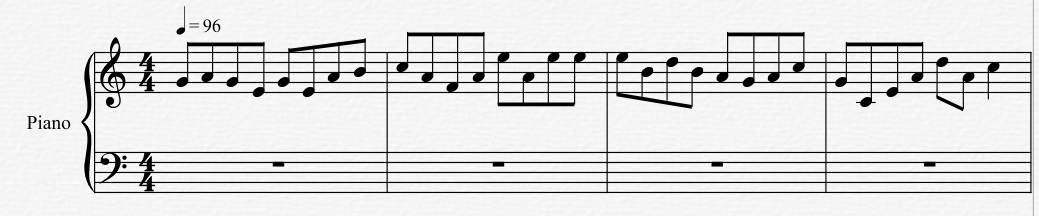
\includegraphics[width=1.0\columnwidth]{eg1.PNG}
            \caption{单旋律实验结果}
        \end{center}
    \end{figure}    
    从实验结果来看,生成的样例中所有音都在C大调音阶中,旋律音程不超过纯五度且不出现增四度,其结尾落在C大调主音上,并是一个长音。可以看到上例中音程行进平稳,旋律线有起伏,但缺乏节奏变化。\par
    此外,我们还尝试了将C大调音阶的要求进一步收紧为五声音阶,希望制作出有民乐特色的音乐,实验结果验证了我们的目标,生成的音乐如下。
    \begin{figure}[H]
        \begin{center}
            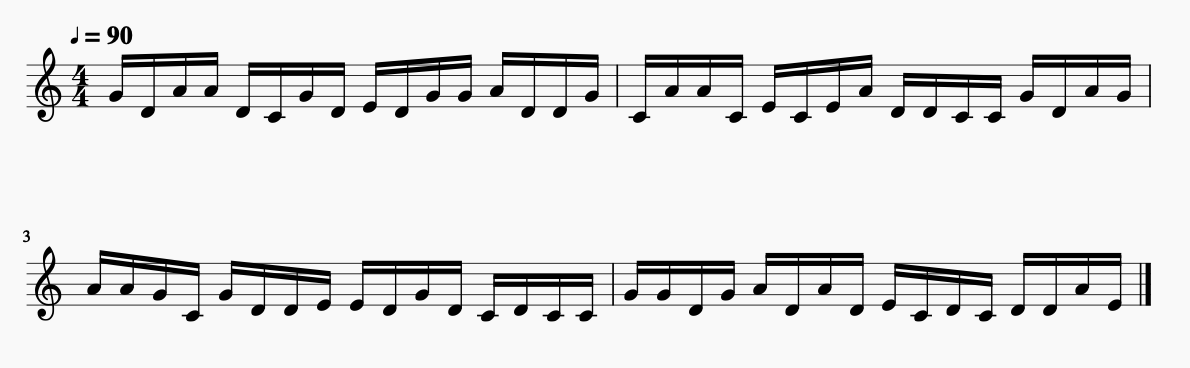
\includegraphics[width=1.0\columnwidth]{five.png}
            \caption{五声音阶实验结果}
        \end{center}
    \end{figure} 

    \subsection{二音对一音}
    二音对一音基本对位是复调的基础之一,相比单旋律音乐有着较多的乐理限制,诸如高声部要比低声部平稳,双声部间的配和,强音和谐,不能使用平行五度行进,连续模进等。我们在程序中实现了这些限制要求。实验得到的实例如下。
    \begin{figure}[H]
        \begin{center}
            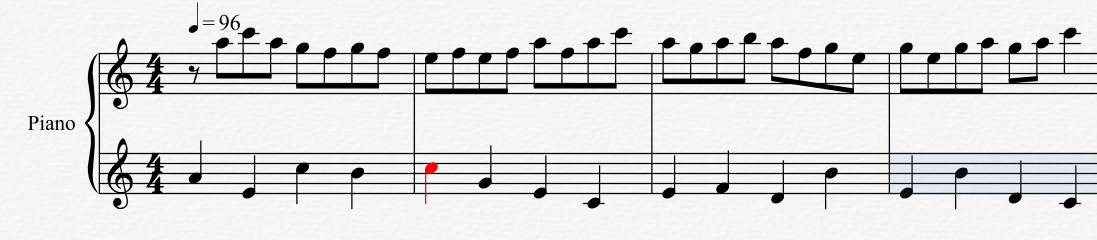
\includegraphics[width=1.0\columnwidth]{eg2.PNG}
            \caption{二音对一音实验结果}
        \end{center}
    \end{figure}
    \begin{figure}[H]
        \begin{center}
            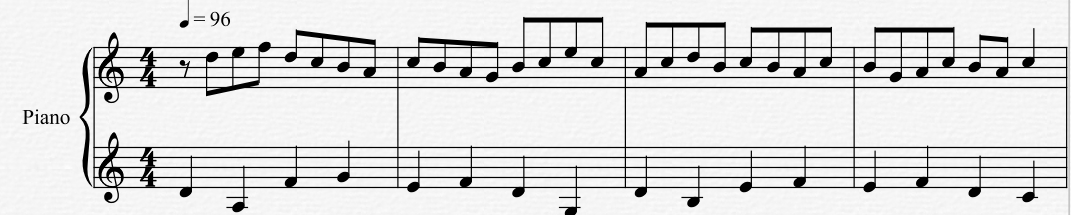
\includegraphics[width=1.0\columnwidth]{eg3.PNG}
            \caption{二音对一音的另一个实验结果}
        \end{center}
    \end{figure}
    实验得到的两个样本满足了二音对一音的乐理要求,其节奏型固定。略有欠缺在于两声部虽然满足和谐关系,但在旋律上的相似性还有所不足,相似的形状并没有带来旋律的熟悉感。当然部分原因在于二音对一音不太能体现出这种模仿。

    \subsection{无终卡农}
    与前面两个音乐形式相比,无终卡农给定了节奏型以及一个严格的曲式限制。在无终卡农中,高声部是低声部的五度守调模进,这在音乐中将带来较好的体验,尤其是第一二小节可以明确的听出主题的再现,然而由于所要求的四个小节长度过短,主题没有完整单声部展现的机会。实际上主题不止一小节这导致后两小节需要反复听后才能分辨。
    \begin{figure}[H]
        \begin{center}
            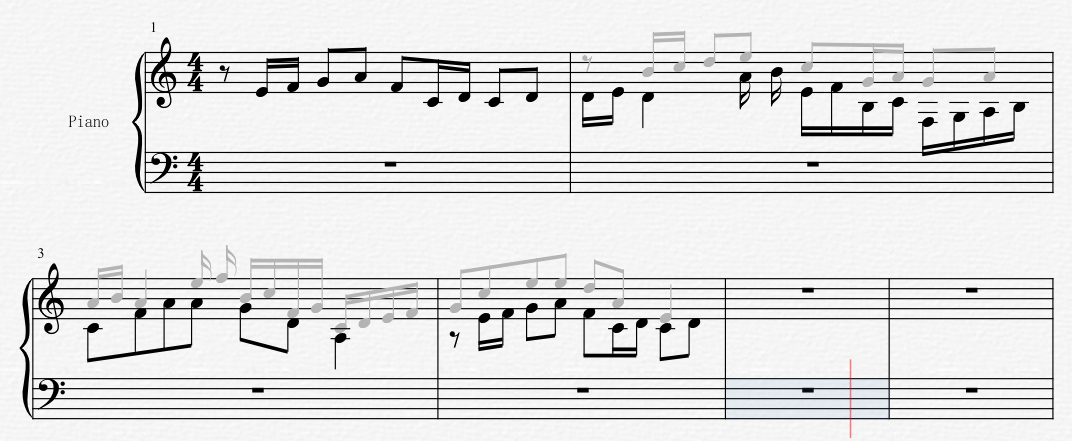
\includegraphics[width=1.0\columnwidth]{eg4.PNG}
            \caption{无终卡农实验结果}
        \end{center}
    \end{figure}
    \begin{figure}[H]
        \begin{center}
            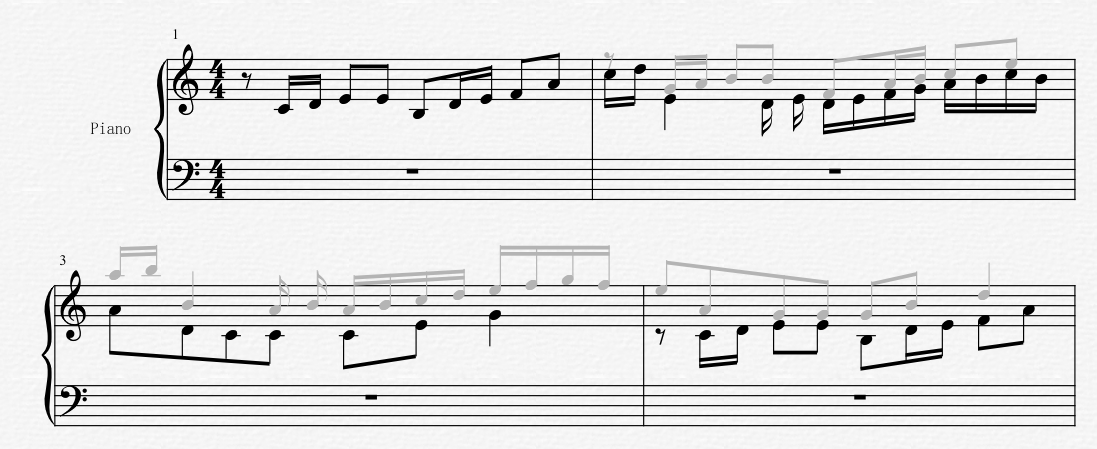
\includegraphics[width=1.0\columnwidth]{eg5.PNG}
            \caption{无终卡农的另一个实验结果}
        \end{center}
    \end{figure}
    面向无终卡农设计的适应度函数与二音对一音基本相同,但此时的强音和谐被改成了同时发出的音和谐,而大量的经过音等不做限制。同时,注意无终卡农的曲式限制使得上述旋律(去掉第一小节)首位相连以后可以无限延续下去,即这是没有中止式的限制的;并且,与单旋律和基础对位不同。\par
    实验中我们还观察到一个有趣的现象,这两首样例的适应度函数均未能降到零即收敛。我们认为这体现了适应度函数不同项间所加的权值的重要性。程序中,和谐音程和调性约束的惩罚力度大于其他。这是由于这两项对听感影响更大,而在适应度函数不能达到零时我们需要优先使它们被满足。

    \subsection{对比式二声部}
    
    \begin{figure}[H]
        \begin{center}
            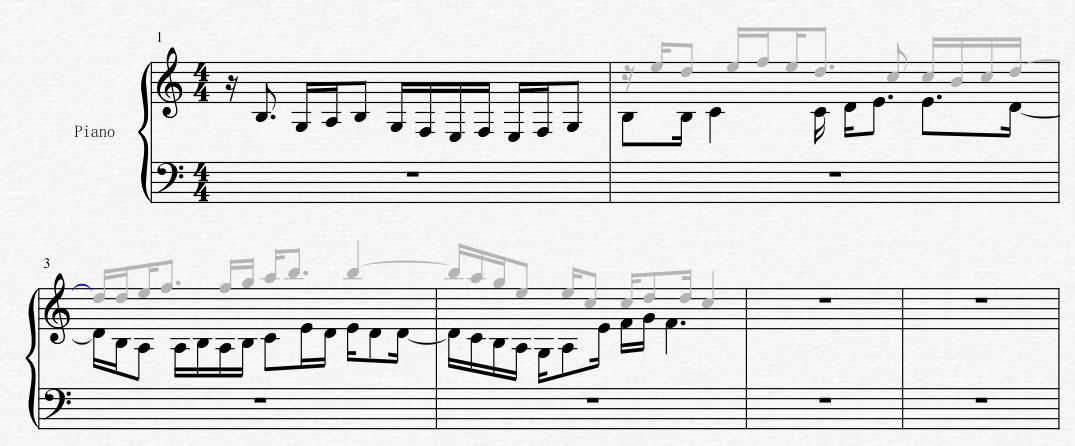
\includegraphics[width=1.0\columnwidth]{eg6.PNG}
            \caption{对比式二声部实验结果}
        \end{center}
    \end{figure}
    首先,在本次实验中,适应度函数仍没有达到零,这意味着可以通过改变适应度函数中不同项的得分来调整总体效果。比如加大和谐音程的分值则会使产生的旋律优先满足和谐音程的条件。\par
    其次,这个生成采用了不给定节奏型也不严格限制高低声部关系的方式。那么想要达到好听的效果则需要高低声部在满足音程和谐以外还应有一些关联而不是完全无关。采用了两部分适应度函数,而它们是可修改的。它们曾在单旋律中给出过实现。分别是控制某小节中延长音的个数和控制两旋律间的行进关系。观察实验结果可以发现,高低声部往往在一个声部音较为密集是另一声部较为稀疏,这使得某一声部的旋律得以展现,这是控制小节中延长音个数带来的效果,想要获得不同的效果则可以通过改变延长音数量配比或是采用给定节奏型的方式,这在无终卡农中实现。\par
    同时,观察实验结果,可以发现高声部和低声部(差一小节,即低声部第一小节开始和高声部第二小节开始)旋律的行进方向基本相似,这将带来一定的主题复现效果。在这个程序中采用了最弱的约束即仅要求行进方向不相反,而不限制具体的旋律音程关系。更严格的方法即不仅限制行进方向,且限制行进的音程也要相似(这曾经似乎在二音对一音中实现过,当时效果不佳)。最严格的方式则是在无终卡农中实现的守调模进(严格模进与音在调上冲突)。\par \
    事实上,我们发现对于单旋律,仅需要满足旋律音程是和谐的,在无节奏型的情况下(即稳定没有延长音),就不难听。故而一段合适的旋律在音程和谐基础上只需要有合适的节奏,而双声部则额外要求两个声部旋律间有关联能配和。这种配和的关键即在于节奏的配和和旋律的配和(主题的复现也包括旋律的复现和节奏的复现)。通过此程序中的适应度函数,在一定程度上实现了旋律和节奏的配和,在主题复现上则实现了旋律的复现。按照相似的方法可以实现节奏的同时复现(这将进一步向卡农靠拢)。不过主要问题在于仍然不能实现某种意义上的两声部配和,即共同传达情感(主题复现只是最粗糙的方式,重复当然是一样的,但是没有配和)。这一点人工给定的经验适应度函数难以达成。

    \section{\textcolor[rgb]{0,0.3,0.6}{基于机器学习的适应度函数基本框架}}
    由于变异、交叉的具体实现大体类似,作曲遗传算法的核心在于适应度函数的具体实现,可以说,作曲遗传算法的好坏决定于适应度函数的好坏。但适应度函数是一个主观性特别强的内容,除去一些普适性的规律直往外,不同的人依据不同的规则和音乐认知,将给出完全不同的适应度函数,所以我们决定尝试着采用机器学习(Machine Learning)的方式实现适应度函数,通过机器学习来提取旋律中的特征,以此去除人为适应度函数的主观性。具体地说,我们将训练一个分类器(Classifier),将不同的旋律划分为好(1)与不好(0),将旋律被划分为好(1)的概率作为其适应度函数,再利用遗传算法进行作曲(图9)。
    \begin{figure}[H]
    \begin{center}
        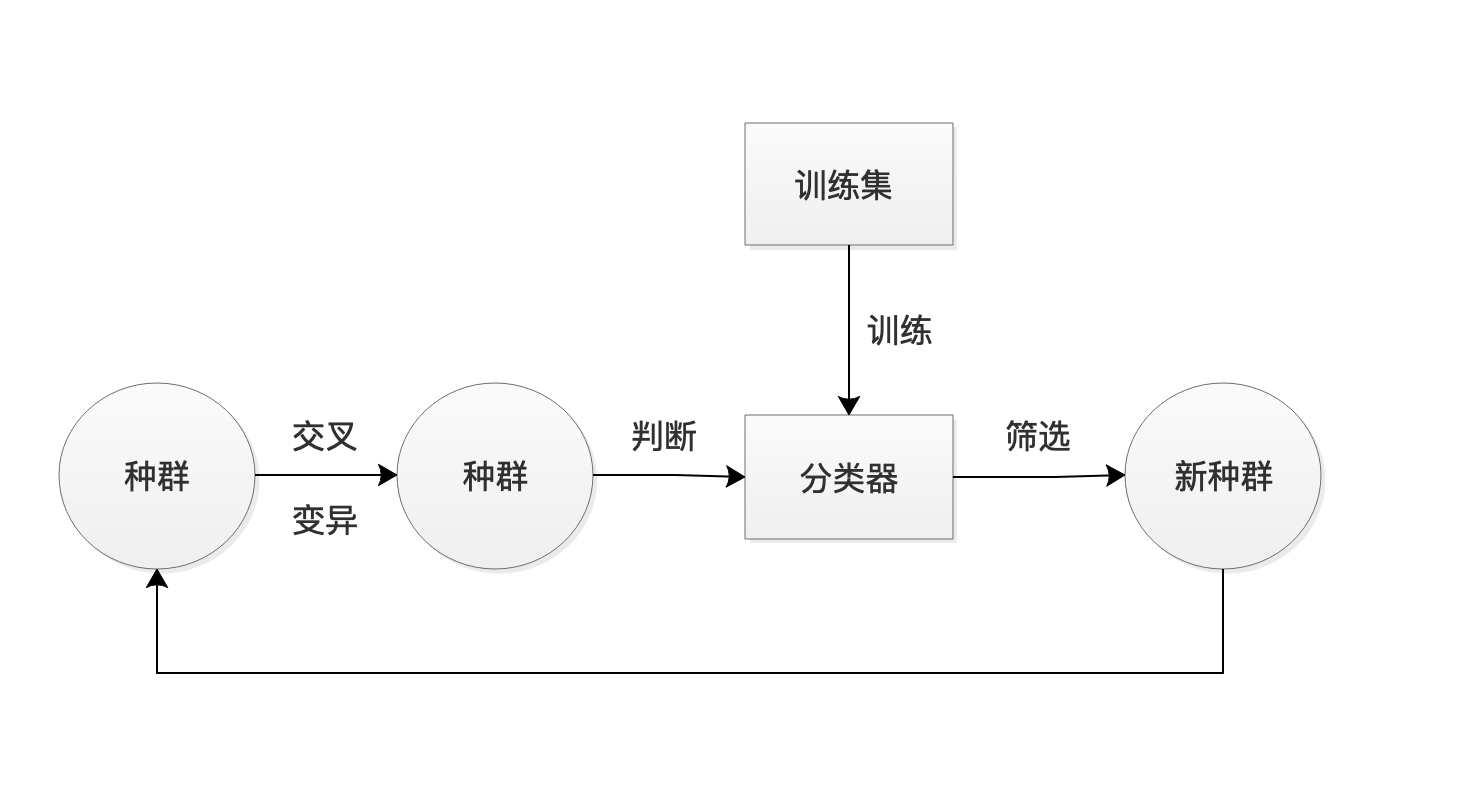
\includegraphics[width=0.7\columnwidth]{flow_chart.png}
        \caption{基本框架}
    \end{center}
    \end{figure}

    \section{\textcolor[rgb]{0,0.3,0.6}{训练集构建}}
    \subsection{MID文件解析}
    相对于其他文件格式,MID文件是较为简单明了,可以明确解析的文件格式。在MID文件中,设置速度、改换音色、增减音轨都是以一个特殊的Event形式存在,特别地,增添音符则以NoteOnEvent,NoteOffEvent两个事件构成,其中NoteOnEvent可视为音符的开始,NoteOffEvent可视为音符的结束,NoteOnEvent和NoteOffEvent均具有三个参数,分别是tick,pitch,velocity,其中tick是时间量(在MID文件中,一般480ticks代表一拍),pitch代表音高(在MID文件中,中央C的pitch为60,每增减一个半音,pitch数值将增减一),velocity则代表力度。三个参数可以被分别读取,这就为我们解析MID文件提供了便利。具体来讲,Python已有现行的库对MID文件进行解析,本文使用的是PythonMIDI,MIDO,PrettyMIDI三个库,三个库均可以在GitHub上找到下载。midi解析的代码见midi\_coding.py文件,在该代码文件中,我们将MID文件转化成了Python 的Numpy二维数组,数组中的每一个值均为一个三维向量[tick,pitch,velocity],在后续的过程中,将使用该向量的形式进行学习。

    \subsection{训练集的选取和构建}
    由于现行的MID文件训练集的资源较少,我们寻找到了134个来自巴赫不同作品的MID文件。出于不同乐器音色不同的考虑,我们将MID文件中的每一个钢琴音轨(MID文件中ProgramChangeEvent的参数在0~7之间代表这个音轨是琴音轨)提取出,共提取出了125个音轨,这些音轨有长有短,而大多数机器学习方法要求输入的向量长度相同,于是我们在每次训练的时候,将随机地从125个音轨中抽取定长的音符片段,形成一个标记为1的训练样本,总共抽取1000个。而标记为0的训练样本则通过随机生成(我们认定随机生成的旋律一定是不好听的或好听的概率很小),将标记为1和标记为0的训练样本合并就得到全体训练集。生成训练集的代码位于代码文件model\_training.py中。


    \section{\textcolor[rgb]{0,0.3,0.6}{学习器的选择和训练}}
    \subsection{传统学习模型}
    本文采取的传统学习模型主要有逻辑斯蒂回归(Logistic Regression,其中代表惩罚项的参数C=100),多层感知机(Multilayer Perceptrons, MLP,其中包含1000个隐藏层,每层包括100个神经元),随机森林(Random Forest,其中代表集成学习分类器个数的参数n\_estimators=100)三种模型。其中逻辑斯蒂回归的原理最为简单,采用的是线性模型和随机森林的原理则稍为复杂,以上三种学习模型的原理可以在任何一本机器学习的教材中找到,此处不再赘述。

    本次使用的传统学习方法都集成于Python的sklearn库中,训练学习器的代码位于代码文件model\_t\ raining.py中,训练好的模型将直接存储在models文件夹中,分别存储为logreg.model,mlp.model,forest.model,方便使用时读取。训练时将全体训练集以3:1的比例划分为训练集和验证集,三种模型在训练集上的分类正确率均较好,但在验证集上逻辑斯蒂回归表现不佳,多层感知机和随机森林则仍旧保持着较高的正确率,某一次训练的训练集、验证集正确率(Accuracy)见表1。
    \makeatletter\def\@captype{table}\makeatother
    \begin{center}
    \caption{不同学习模型的分类正确率表}
    \begin{tabular}{ccc}
    \toprule
    学习模型 & 训练集正确率 & 验证集正确率 \\ 
    \midrule
    逻辑斯蒂回归 & 0.921 & 0.764 \\ 
    多层感知机 & 0.918 &  0.926 \\ 
    随机森林 & 1.0 & 0.995 \\ 
    \bottomrule
    \end{tabular}
    \end{center}

    这点也可以简单地从不同学习模型的特性分析出。对于逻辑斯蒂回归来说,每一个音的tick,pitch,\  velocity三个性质都是一个独立的维度,对于64个音符的片段,就相当于192维的向量,而且这192个维度互相独立,互不影响,没有联系,当使用逻辑斯蒂回归进行分类时,分类器将分别考虑每一个位置上的音符,而并没有考虑音符之间的关系(即各个维度之间的关系),对旋律而言,这种考量是不科学的,旋律的好听与否,在很大程度上取决于其音间关系 (例如音程关系),所以我们可以断言逻辑斯蒂回归这种简单的几乎全线性(惩罚项$||\beta||_2^2$赋予了其一定的非线性性)的模型并不适合用于学习旋律这样维度之间存在或显性或隐性关系的样本。相反由于多层感知机在每经历一次全连接层的线性变化之后都会通过某一个阈值函数(例如RELU,或是tanh函数)对输出的结果进行一定的非线性变换,此时音间关系就有可能被学得,随机森林基于决策树方法,在集成学习的整体框架下,音间关系也是有可能被学习的。

    \subsection{深度学习模型}

    对于旋律特征的学习和提取而言,传统的学习模型仍然具有难以避开的问题。对于一段乐曲而言,例如它的编码是$[a_1,a_2...a_{64}]$,此时我们判断它是“好听的”,对于传统的学习模型,其每个音符的位置时固定的,也就是说,传统学习模型认为只有在$a_1$处于第0个位置,$a_2$处于第1个位置...$a_{64}$处于第63个位置的时候才是好听的,如果我们将乐曲做时间上整体平移,再在头尾适当增补某些音符(例如将编码变为$[a_0,a_1...a_{63}]$),就我们人来说应该大概率也是好听的,但此时传统学习模型训练处的分类器很有可能就认为其“难听”,也就是说,传统学习模型很难学习出旋律的这种“时间平移对称性”的特征。

    据此联想到被广泛用于图像数据处理的卷积神经网络(Convolutional Neural Networks, CNN),由于图像在局部的区域内同样存在平移对称性,而卷积操作可以在一定程度上将这种特征提取出来,那么对于旋律在时间轴上的对称性,利用一维卷积操作应该也可以一定程度上在分类器中保留这种特征。

    在music\_net.py文件中,使用PyTorch库搭建了一个包含多个卷积层、最大池化层和若干全连接层的小型神经网络(MusicNet),具体结构如图10。(输入向量的每一维代表一个音符,一个音符含有3个参数,于是输入的通道数为3,图中以长度为64个音符的旋律举例)
    \begin{figure}[H]
    \begin{center}
        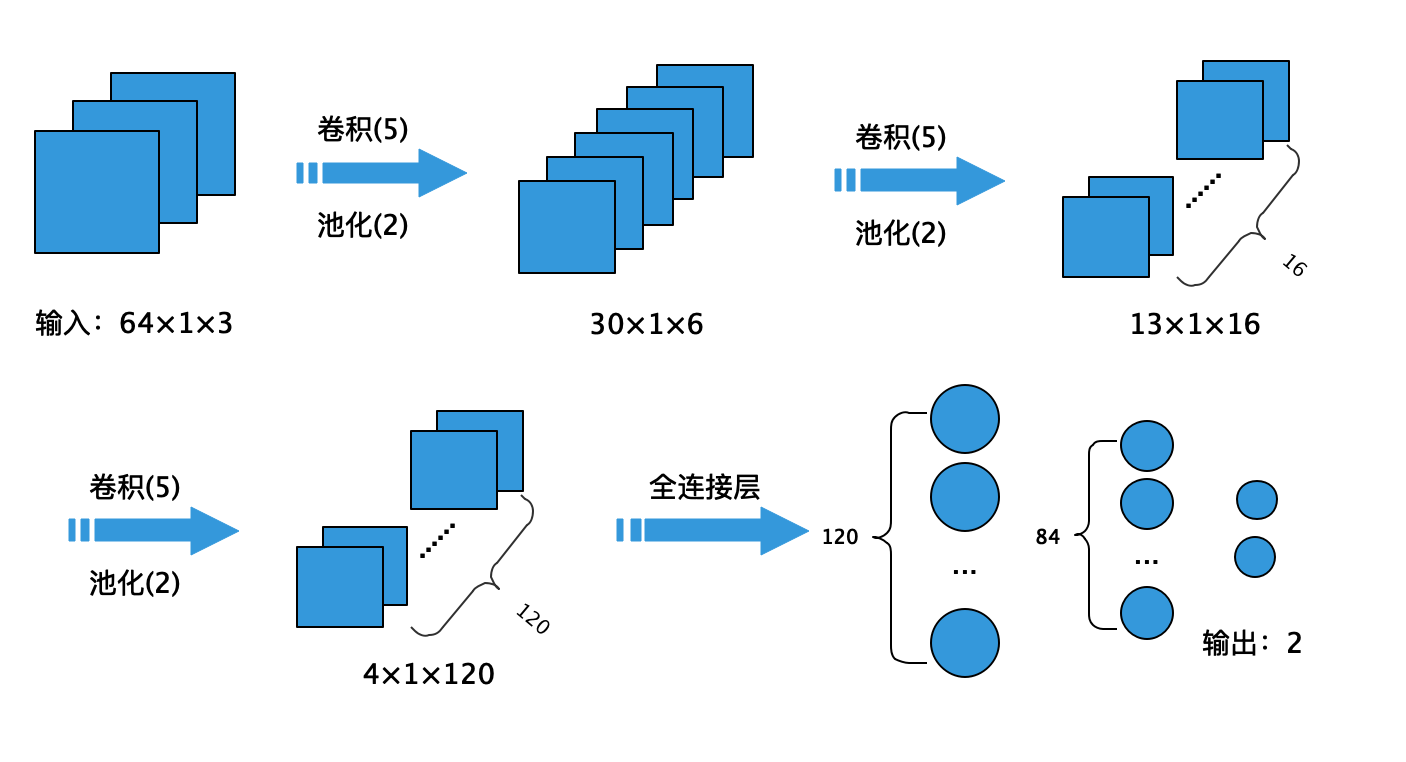
\includegraphics[width=0.7\columnwidth]{CNN_net_structure.png}
        \caption{MusicNet结构}
    \end{center}
    \end{figure}

    该网络以交叉熵(CrossEntropy)为损失函数,采用SGD小批量随机梯度下降方法,学习率为0.001,动量参数momentum为0.9,在前述训练集下以小批量(batch\_size=50)训练50代,此时损失函数已经基本降至0,训练好的网络在训练集和验证集上的分类正确率均在0.995以上。此时将训练好的网络参数存储至models文件夹下的music\_net.tar,方便使用时读取。



    \section{\textcolor[rgb]{0,0.3,0.6}{基于机器学习的遗传算法作曲}}
    遗传算法的整体框架和前述的人工适应度函数所用框架大致相同,由于旋律的具体表现形式不同(此处将音符的时值和力度特性以另外两个维度的形式体现,所以同样长度为64的旋律,人工适应度函数的编码是长度为64的向量,而此处的编码为64行3列的矩阵),所以对各个部分略作修改,具体实现已集成于main.py文件中,变异部分(见Population类的mutation函数)包含单个音符的变异、整体移调、逆行和倒影,并设置变异率为0.1,选择部分则使用遗传算法常用的轮盘赌算法(见Population类的selection函数),计算适应度时则直接用特定的学习器对输入的音符矩阵进行概率预测(predict\_proba,见Individual类的cal\_fitness函数),在实验时规定种群大小为30,迭代代数为1000代,1000代之后选取种群中最好的个体,用集成于midi\_coding.py文件中的reconversion函数将其转化为midi文件输出。

    实验中在每一代提取其个体适应度的平均值,作图如图11-图14所示。

    \begin{figure}[H]
    \begin{minipage}[t]{0.5\linewidth}
    \centering
    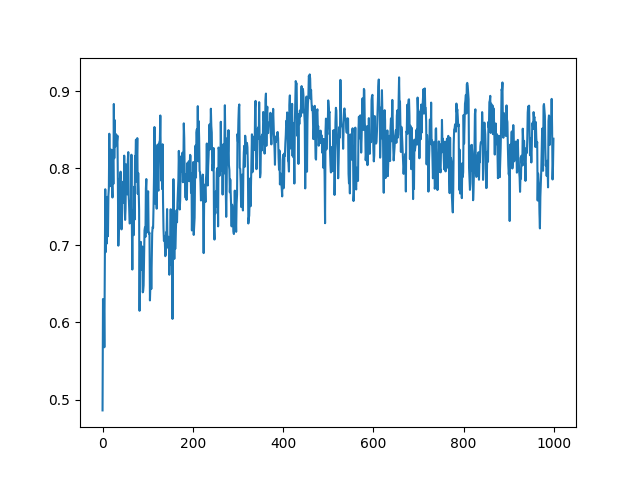
\includegraphics[width=3in]{output_logreg.png}
    \caption{Logistic Regression}
    \label{fig:side:a}
    \end{minipage}%
    \begin{minipage}[t]{0.5\linewidth}
    \centering
    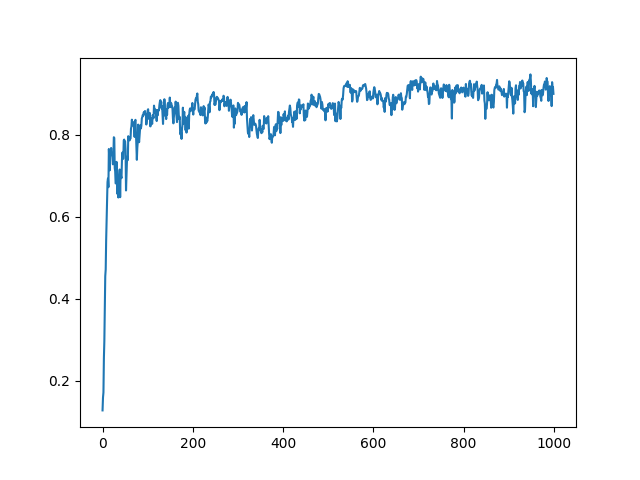
\includegraphics[width=3in]{output_mlp.png}
    \caption{MLP}
    \label{fig:side:b}
    \end{minipage}
    \end{figure}

    \begin{figure}[H]
    \begin{minipage}[t]{0.5\linewidth}
    \centering
    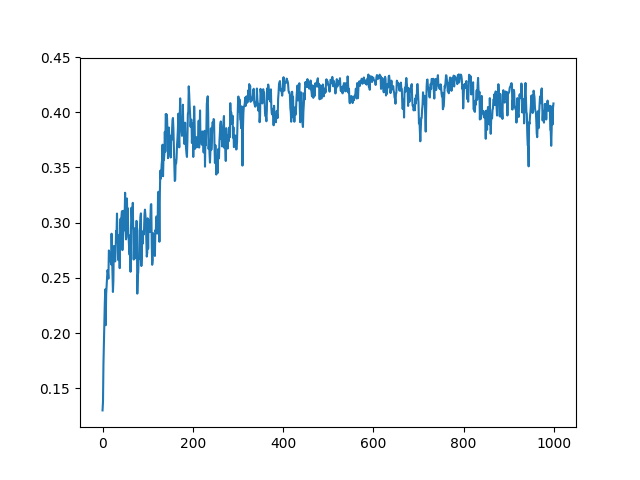
\includegraphics[width=3in]{output_forest.png}
    \caption{Random Forest}
    \label{fig:side:a}
    \end{minipage}%
    \begin{minipage}[t]{0.5\linewidth}
    \centering
    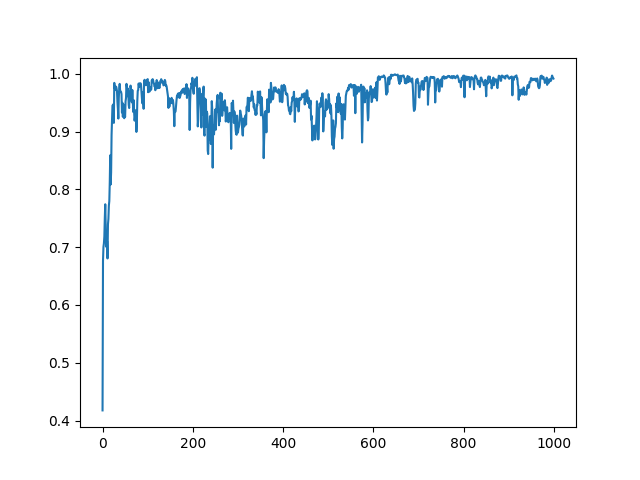
\includegraphics[width=3in]{output_cnn.png}
    \caption{CNN}
    \label{fig:side:b}
    \end{minipage}
    \end{figure}

    从这四幅图中可以发现一些有意思的现象。在迭代1000代之后,四种学习模型都已经达到了一个稳定值,由于变异的存在,以稳定值为中心上下波动。对于逻辑斯蒂回归,它的迭代起点相当高(接近0.5),这就说明在种群初始化时,我们随机生成的音符片段被认为是“好听的”概率在0.5以上,这显然是荒谬的,并且其在后续迭代的过程中上下波动相当剧烈,这就说明在小范围变异(变异率为0.1,这是一个相对较小的值)的作用下其种群的分类概率可以发生显著波动,这显然也不符合旋律片段将在遗传算法作用下最终收敛的特性。MLP和CNN由于原理大体类似,在遗传算法作用下显示出了相似的图像,在迭代后期波动较小,有收敛至1(说明其可以产生一个分类器认为是“绝对好听”的旋律)的趋势,CNN已经接近收敛于1。随机森林则在迭代1000次以后,最高的平均适应度仍然不及0.45,换言之,在迭代1000次后仍然不能产生一个令随机森林分类器“满意”的个体,这说明随机森林对“好”的要求较为严苛,限制较多,随机森林的学习模型很有可能存在“过拟合”的风险。

    在经过试验之后,产生的乐曲片段都已经转化成MIDI文件存储在output\_melody文件夹中,其五线谱如图15-图18所示。
    \begin{figure}[H]
    \begin{center}
        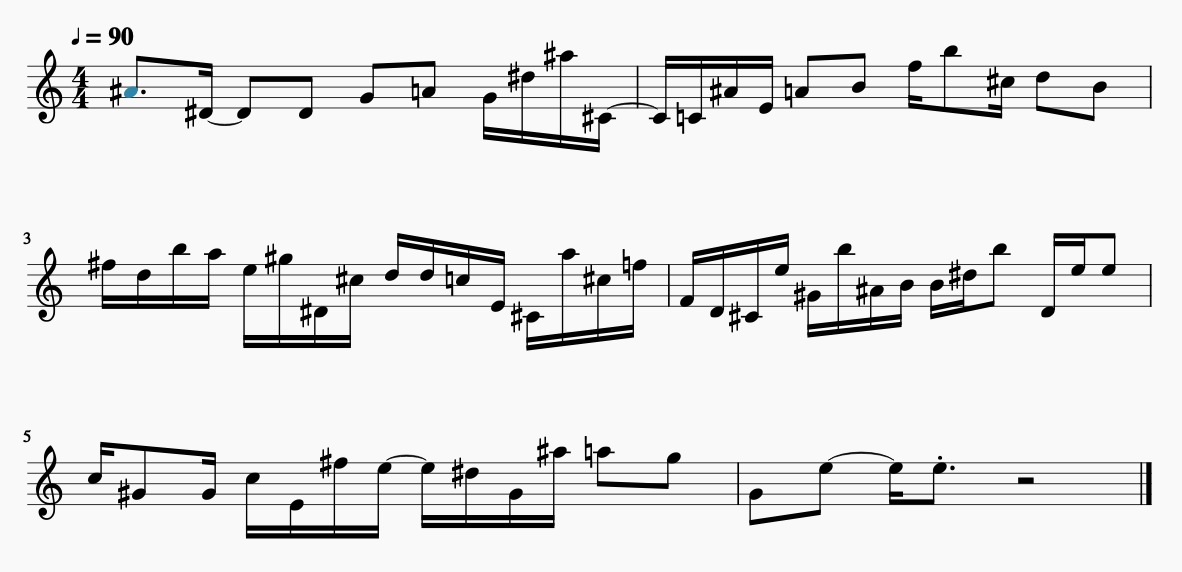
\includegraphics[width=1.0\columnwidth]{output_logreg_melody.png}
        \caption{Logistic Regression}
    \end{center}
    \end{figure}

    \begin{figure}[H]
    \begin{center}
        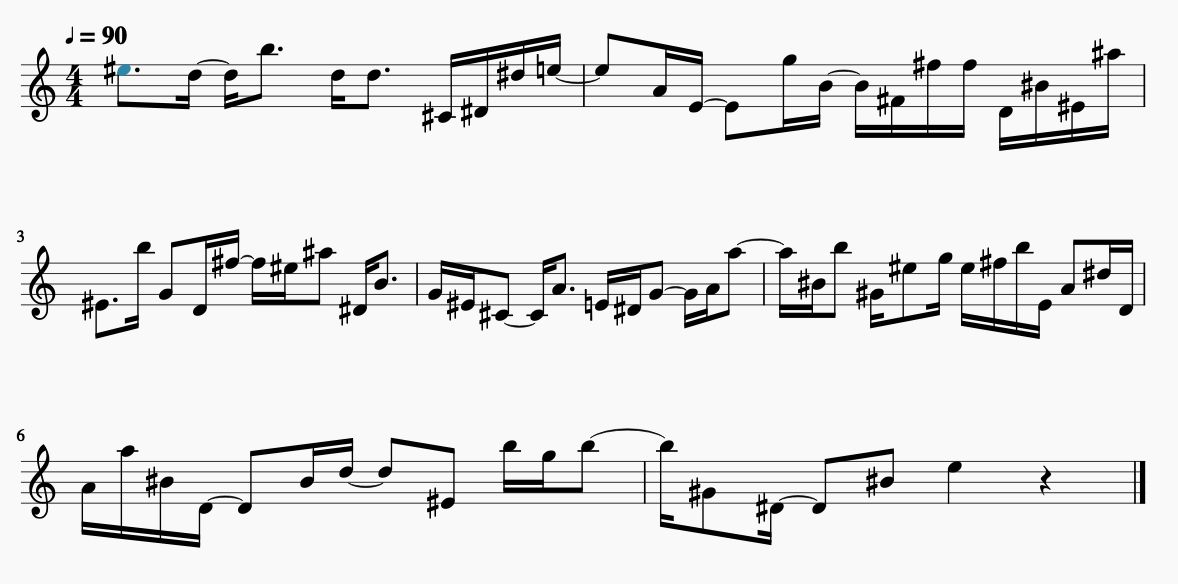
\includegraphics[width=1.0\columnwidth]{output_mlp_melody.png}
        \caption{MLP}
    \end{center}
    \end{figure}

    \begin{figure}[H]
    \begin{center}
        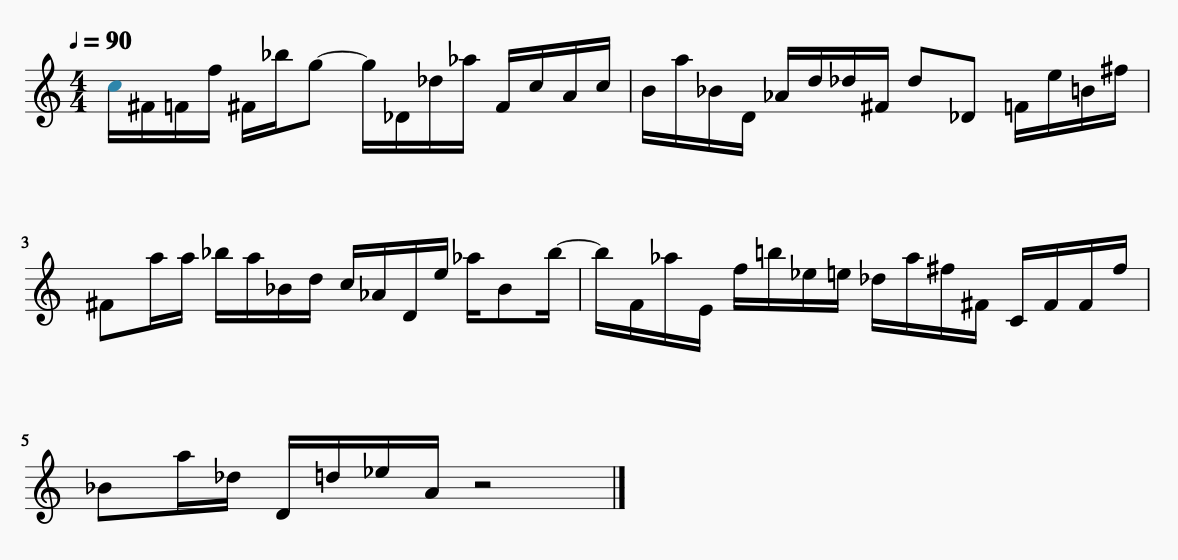
\includegraphics[width=1.0\columnwidth]{output_forest_melody.png}
        \caption{Random Forest}
    \end{center}
    \end{figure}

    \begin{figure}[H]
    \begin{center}
        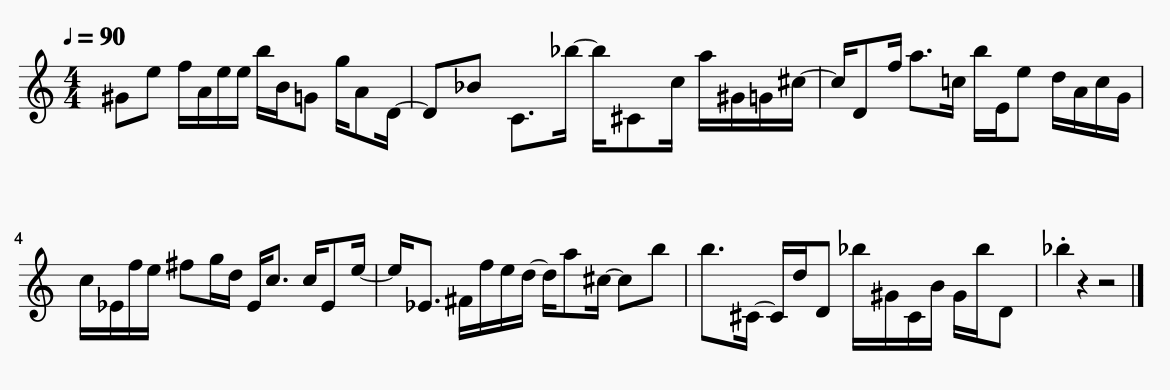
\includegraphics[width=1.0\columnwidth]{output_cnn_melody.png}
        \caption{CNN}
    \end{center}
    \end{figure}

    可以说,这四段旋律都不能算好听,甚至有些刺耳 ,经过对这几段旋律的简单,我们认为其不好听的原因可能有以下几个:
    \begin{itemize}
        \item 节奏型乱。这点可以追溯到我们训练集构建的部分,在训练集构建的过程中,我们所选取的134个MID文件具有不同的节奏型和节拍,并且我们在构建训练集的时候是随机截取的定长音符的音轨片段,而不是以小节为片段进行截取,而节奏型与小节的划分具有密切联系,这使得在我们的训练集中,时值(tick)这一维度的数据是近似随机的,在用学习模型进行特征提取的时候提取出的特征也是近似随机的,最终产生旋律的节奏型效果并不好。这个问题的解决方案是按照完整乐句截取训练集,但对于MID文件格式,由于其没有记录节拍、小节划分的数据,所以分割乐句的任务具有难度,目前除了手动筛选以外没有其他的解决方案,所以节奏型上很难再进行改良。
        \item 音程跳跃大,听起来不稳定。我们对某次实验中四种学习器输出的旋律编码进行了差分,取绝对值之后对其进行了统计,绘制直方图如图19-22所示(横轴代表半音数,纵轴代表其出现次数)。我们可以较为明显地看到,逻辑斯蒂回归的各个半音音程出现的较为平均,大跳跃(指半音数大于等于12,即8度以上)音程也占比比较高,这和前面分析的逻辑斯蒂回归并不能处理音间关系的推论是符合的。对于剩下的三种学习模型,大音程占比变少,但仍然普遍存在,占比最高的音程普遍位于5~8左右,可能对应纯四度(对应5个半音)、纯五度音程(对应7个半音 ),但不可避免地产生增四度(对应6个半音)、减五度(对应6个半音)这种并不使人愉悦的音程关系。而使人产生稳定感的大二度、小二度或是重音虽有出现,频率不大,这使得悦耳旋律中经常出现的连续上下行在输出旋律中很少出现,也就是说,在输出的旋律之中存在“忽上忽下”的跳跃情形,各个音之间较为零散,构不成完整的乐句,更不要提“旋律复现”。对于这一点,我们能做的改良仍然是有限的,由于机器学习算法的复杂性,我们不能很直观地得知机器到底从训练集中提取到了什么特征,我们也无从知晓一个具体的学习器是如何处理对应的音间关系的,无从知晓分类器是仅仅处理相邻两个维度的关系,还是考虑到了更高阶的维度联系。我们能够想到的改良方案是将输入向量进行音高差分之后与原来的编码向量合并,将相邻两个音的音间关系作为独立维度进行训练学习,但尝试的效果并不佳,可能需要考虑更高阶的音程关系。
    \begin{figure}[H]
    \begin{minipage}[t]{0.5\linewidth}
    \centering
    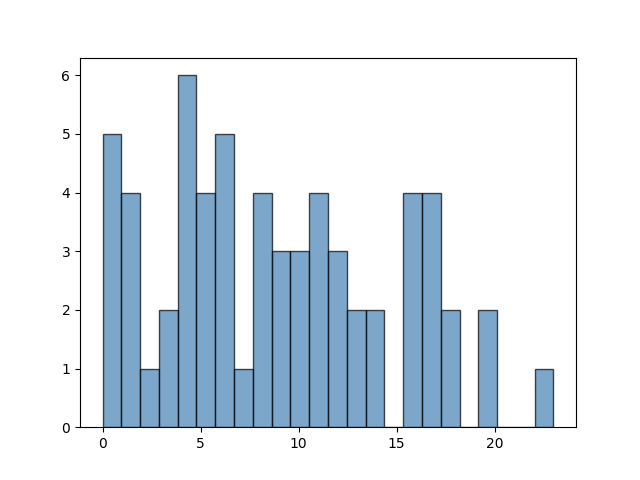
\includegraphics[width=3in]{output_logreg_hist.png}
    \caption{Logistic Regression}
    \label{fig:side:a}
    \end{minipage}%
    \begin{minipage}[t]{0.5\linewidth}
    \centering
    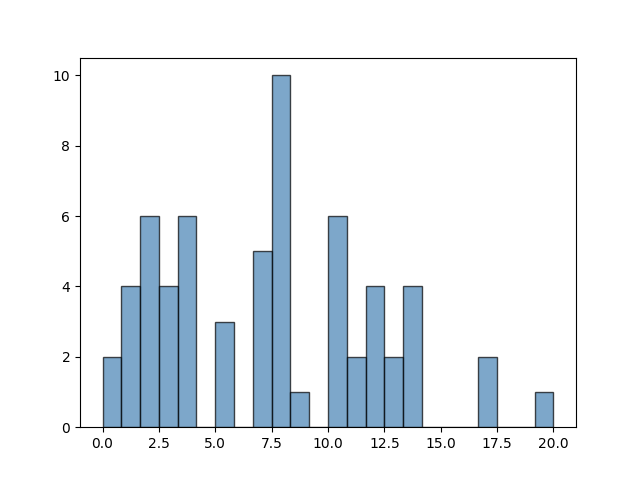
\includegraphics[width=3in]{output_mlp_hist.png}
    \caption{MLP}
    \label{fig:side:b}
    \end{minipage}
    \end{figure}

    \begin{figure}[H]
    \begin{minipage}[t]{0.5\linewidth}
    \centering
    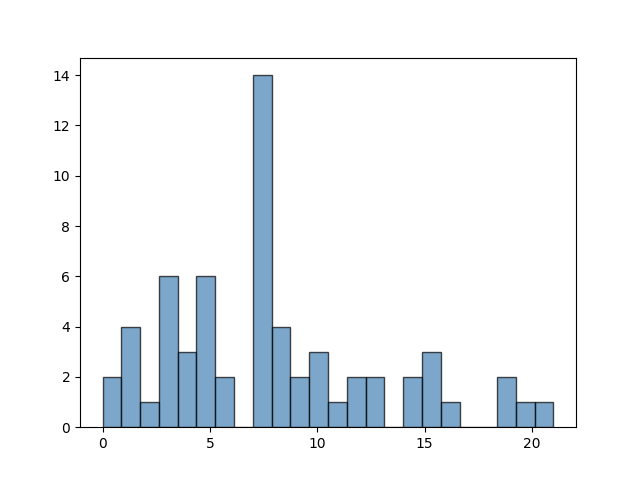
\includegraphics[width=3in]{output_forest_hist.png}
    \caption{Random Forest}
    \label{fig:side:a}
    \end{minipage}%
    \begin{minipage}[t]{0.5\linewidth}
    \centering
    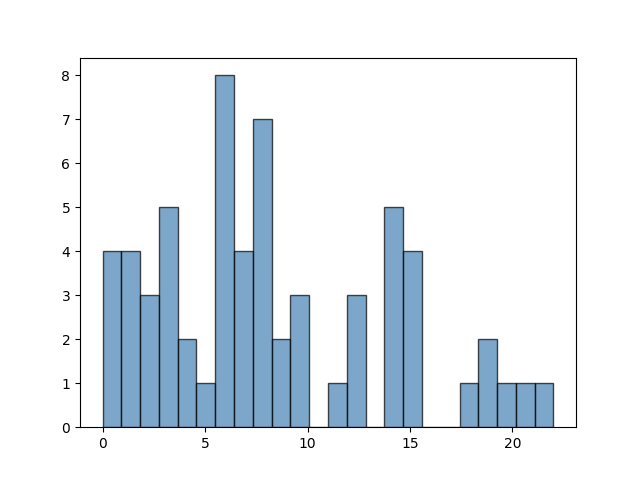
\includegraphics[width=3in]{output_cnn_hist.png}
    \caption{CNN}
    \label{fig:side:b}
    \end{minipage}
    \end{figure}
    \item 不在调上的音占比高。考虑到训练集的作品C大调占了多数,从C大调的角度去分析,在某一次实验中  四种方法不在调上的音符占比如表2。
    \makeatletter\def\@captype{table}\makeatother
    \begin{center}
    \caption{不同学习模型的输出旋律调性分析}
    \begin{tabular}{cccc}
    \toprule
    学习模型 & 音符总数 & 在调式中的音符个数 & 调性音符占比 \\ 
    \midrule
    逻辑斯蒂回归 & 64 & 40 & 62.5\% \\ 
    多层感知机 & 64 &  34 & 53.1\% \\ 
    随机森林 & 64 & 38 & 59.4\%\\ 
    卷积神经网络 & 64 & 47 & 73.4\% \\ 
    \bottomrule
    \end{tabular}
    \end{center}

    调性音符占比呈现出了较强的随机性,旋律并没有对调性音符产生强烈的偏好,这可能也与我们选取训练集中含有部分非大调的乐曲有关,也有可能是机器学习算法本身的缺陷使旋律的调性特征没有被习得。我们同样可以对其中出现的音高做统计,绘制直方图如图23-26,可以看到,算法本身并没有对某些音具有明显的偏好,统计呈现较强的均匀性和随机性。关于这点,我们曾经尝试在在生成种群个体时仅仅使用C大调上的音,变异也限制于C大调,这时候如果使用相同的分类器进行迭代,迭代1000代之后种群的平均适应度仍然很难达到0.7,也就是说如果将音局限于C大调,分类器将不认为它是一段好听的旋律。值得一提的是,如果将个体限制在五声音阶(CDEGA)上,所有音之间的音程关系都较好,此时就算随机生成的旋律也非常悦耳,但分类器仍然不认为其是好听的。

    \begin{figure}[H]
    \begin{minipage}[t]{0.5\linewidth}
    \centering
    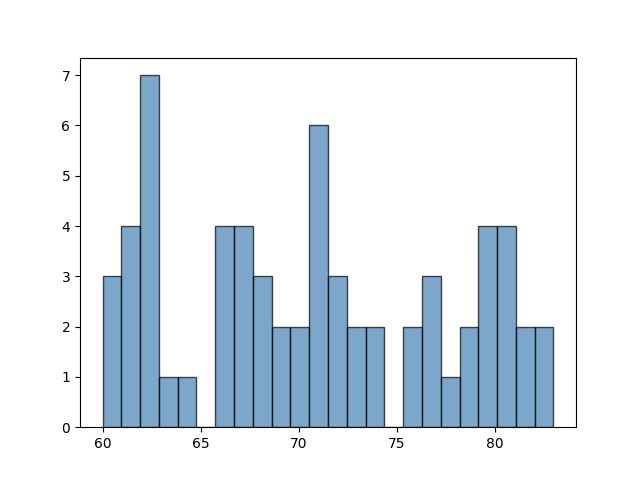
\includegraphics[width=3in]{output_logreg_hist_1.png}
    \caption{Logistic Regression}
    \label{fig:side:a}
    \end{minipage}%
    \begin{minipage}[t]{0.5\linewidth}
    \centering
    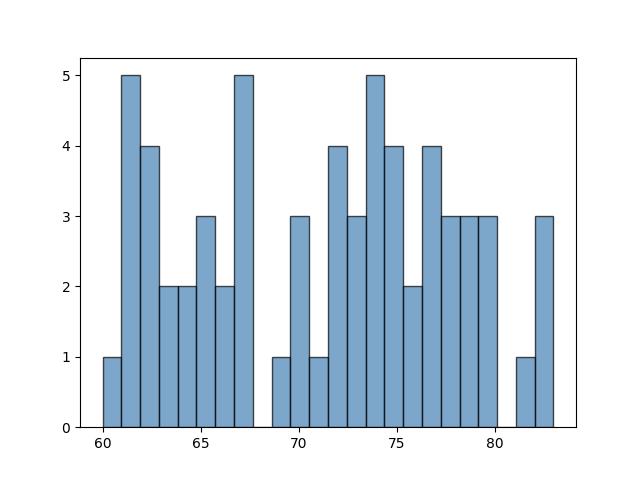
\includegraphics[width=3in]{output_mlp_hist_1.png}
    \caption{MLP}
    \label{fig:side:b}
    \end{minipage}
    \end{figure}

    \begin{figure}[H]
    \begin{minipage}[t]{0.5\linewidth}
    \centering
    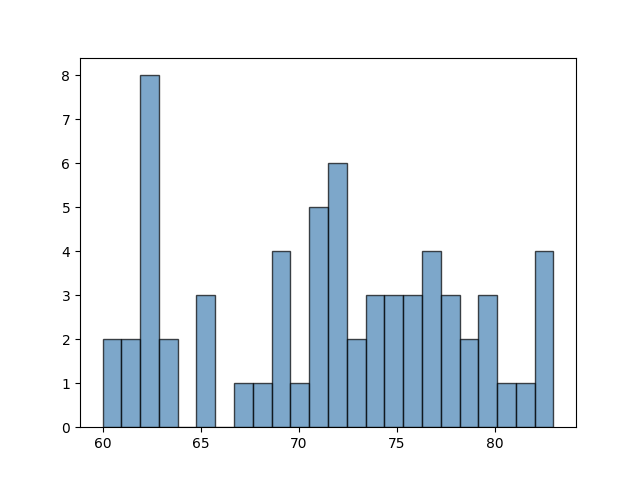
\includegraphics[width=3in]{output_forest_hist_1.png}
    \caption{Random Forest}
    \label{fig:side:a}
    \end{minipage}%
    \begin{minipage}[t]{0.5\linewidth}
    \centering
    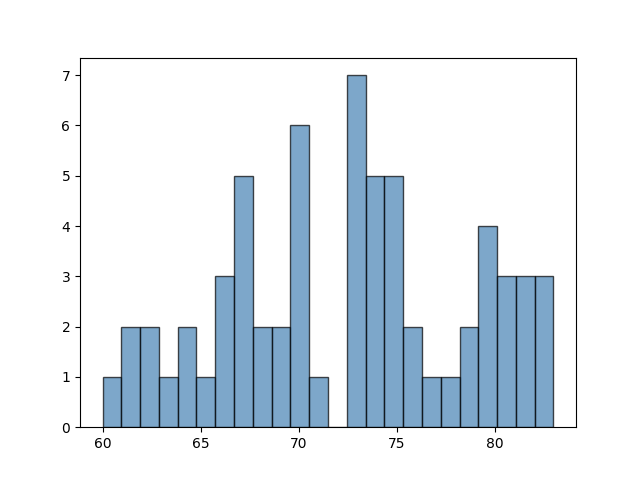
\includegraphics[width=3in]{output_cnn_hist_1.png}
    \caption{CNN}
    \label{fig:side:b}
    \end{minipage}
    \end{figure}
    \end{itemize}

    \section{\textcolor[rgb]{0,0.3,0.6}{算法效率分析}}

    由于机器学习算法已经封装在sklearn库中,它们的时间复杂度由机器学习方法本身决定,因此,机器学习模型和训练集规模确定后,算法的时间复杂度和效率是确定的,我们不必对于这些封装完全的算法做更多时间效率上的优化。本文中所涉及的部分机器学习算法的时间复杂度列于下表。
    \begin{center}
        \begin{tabular}{ccc}
            \toprule
            算法&时间复杂度&注释\\
            \midrule
            % 逻辑斯蒂回归&$O()$&\\
            % 多层感知机&$O()$\\
            随机森林&$O(N\times M\times D)$&N是样本的大小,M是特征的数量,D是树的深度\\
            卷积神经网络&$O(n\times k_1 + \sum k_n)$&$k_i$为模型的第$i$层维度\\
            \bottomrule
        \end{tabular}
    \end{center}
    此外,我们不妨考察一下筛选算法对于程序时间效率的影响。在使用同一个适应度函数的情况下,我们通过实验测试了轮盘赌算法和贪心法收敛的速率。下图给出了每轮筛选出的子代的适应度平均值随迭代筛选轮次的波动,蓝色曲线代表贪心法,橙色曲线代表轮盘赌算法。从实验结果我们可以看出,贪心法收敛的速度和筛选出的子代质量要远远高于轮盘赌的结果,但是,经历较少轮次收敛也存在着进化不充分,容易落入初始种群一个小邻域内的局部最优解的可能。为此,我们需要尽量采用随机生成的初始种群,以规避取得局部最优解的风险。

    \begin{figure}[H]
        \centering
        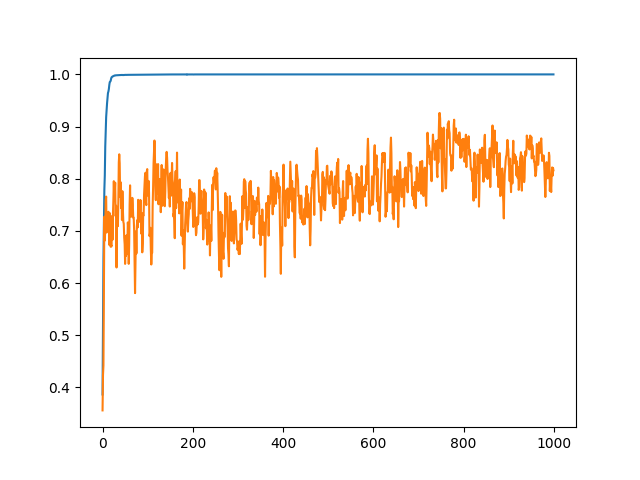
\includegraphics[width=3in]{compare.png}
        \caption{筛选算法对程序时间效率的影响}
        \label{}
    \end{figure}

    \section{\textcolor[rgb]{0,0.3,0.6}{总结}}

    本文中我们报道了两种构造遗传算法作曲中适应度函数的方法,分别是利用乐理知识经验和机器学习方法构造适应度函数。\par
    基于乐理知识的经验适应度函数可以充分利用现有的乐理知识,量化人对音乐“好听”的感受,实现创作出“好听”乐曲的目的。这样的音乐通常带有一定的适应度函数编制者个人色彩。此外,我们还尝试利用乐曲的马尔可夫矩阵来表征乐曲的旋律性质,加进适应度函数中评分,但结果变化不大,我们猜测这和音乐的马氏性并不完全有关。\par
    在构造基于机器学习的适应度函数过程中,我们旨在通过机器学习算法提取悦耳旋律的特征,构建分类器作为适应度函数的判据来排除人工适应度函数的主观性,或去发掘一些人无法感知的音乐特征。最终给出的旋律并不理想,这可能与训练集的选取,分类器的构建相关,由于机器学习算法的“黑箱特性”,我们无法直观地理解机器在分类时的判断依据,后续改良只能通过调整参数,改变训练集来逐步摸索实现。在后续的实验中,我们尝试着手动筛选了20个节奏型相近、同属于C大调、音乐风格相近的完整乐句,但由于20个样本的训练集过小,训练过程的随机性较大,产生的结果也并不理想。要使机器学习适应度函数真正能够写出悦耳动听的旋律还需要后续的改良。

    \section{\textcolor[rgb]{0,0.3,0.6}{致谢}}
    以下排名不分先后。\par 
    感谢王杰老师和助教们本学期的教学与指导。\par
    感谢关震岳同学完成了算法复杂度分析部分内容,以及对机器学习算法的改进。\par 
    感谢李宇轩同学完成了算法复杂度分析部分内容,以及Matlab语言程序设计支持。\par 
    感谢林潇涵同学完成了机器学习适应度函数的Python实现,以及机器学习部分内容的写作。\par
    感谢胡泽昕同学完成了经验适应度函数的C语言实现,以及经验适应度函数部分内容的写作。\par
    感谢张天越同学完成了移调、倒影、逆行部分的JavaScript代码实现,以及对机器学习算法的改进。\par 
    感谢施朱鸣同学完成了论文写作与\LaTeX 排版,以及对团队提出的几项算法的改进。\par
    通讯邮箱shizhuming@pku.edu.cn。

    \section{\textcolor[rgb]{0,0.3,0.6}{参考文献}}
    Järvelainen H. Algorithmic musical composition. 2000\\
\end{document}